\documentclass[10pt]{article}
\usepackage[margin=1in]{geometry}
\usepackage{amsmath,amssymb}
\usepackage{graphicx}
\usepackage{listings}
\usepackage{xcolor}
\usepackage{tikz}
\usepackage{tcolorbox}
\usepackage{hyperref}

% Colors
\definecolor{codegreen}{rgb}{0,0.6,0}
\definecolor{codegray}{rgb}{0.5,0.5,0.5}
\definecolor{codepurple}{rgb}{0.58,0,0.82}
\definecolor{backcolour}{rgb}{0.95,0.95,0.92}

% Code style
\lstdefinestyle{mystyle}{
    backgroundcolor=\color{backcolour},   
    commentstyle=\color{codegreen},
    keywordstyle=\color{magenta},
    numberstyle=\tiny\color{codegray},
    stringstyle=\color{codepurple},
    basicstyle=\ttfamily\footnotesize,
    breakatwhitespace=false,         
    breaklines=true,                 
    captionpos=b,                    
    keepspaces=true,                 
    numbers=left,                    
    numbersep=5pt,                  
    showspaces=false,                
    showstringspaces=false,
    showtabs=false,                  
    tabsize=2
}
\lstset{style=mystyle}

% Custom commands
\newcommand{\question}[1]{\vspace{0.5em}\noindent\textbf{Q: #1}\vspace{0.3em}}
\newcommand{\exercise}[1]{\vspace{0.5em}\noindent\textbf{Exercise: #1}\vspace{0.3em}}
\newcommand{\think}[1]{\vspace{0.3em}\noindent\textit{Think: #1}\vspace{0.3em}}
\newcommand{\theoryhint}[1]{
    \begin{tcolorbox}[colback=blue!5!white,colframe=blue!60!black,title=Theory Hint]
    #1
    \end{tcolorbox}
}
\newcommand{\checkpoint}[1]{
    \begin{tcolorbox}[colback=yellow!10!white,colframe=yellow!75!black,title=Checkpoint]
    #1
    \end{tcolorbox}
}
\newcommand{\discovery}[1]{
    \begin{tcolorbox}[colback=green!5!white,colframe=green!75!black,title=Discovery]
    #1
    \end{tcolorbox}
}
\newcommand{\realworld}[1]{
    \begin{tcolorbox}[colback=orange!5!white,colframe=orange!75!black,title=Real World Example]
    #1
    \end{tcolorbox}
}

\title{Week 5: Attention Is All You Need - Transformers\\
\large Discovery-Based Learning with Guided Exploration}
\date{}

\begin{document}
\maketitle

\section*{Learning Journey}
Today we'll discover the architecture behind ChatGPT, BERT, and modern AI. Imagine a classroom where everyone can talk to everyone else simultaneously - that's the transformer revolution!

\section*{Learning Objectives}
By the end of this session, you will:
\begin{itemize}
    \item Understand why RNNs have fundamental limitations
    \item Discover self-attention from first principles
    \item Design the multi-head attention mechanism
    \item Build a complete transformer architecture
    \item Master positional encodings
\end{itemize}

\hrule
\vspace{1em}

\section{Part 1: The Sequential Processing Problem (10 minutes)}

\subsection{The Telephone Game}

\theoryhint{
RNNs process sequences one element at a time, like a game of telephone. Each step depends on the previous one, creating a bottleneck. Information can degrade as it passes through many steps, and we can't process step 10 until we've processed steps 1-9.
}

\realworld{
\textbf{RNN (Sequential)}: Like reading a book one word at a time with your finger\\
\textbf{Transformer (Parallel)}: Like seeing the whole page at once
}

\exercise{Let's process this sentence with an RNN. Mark the dependencies:}

``The student who studied hard and completed all assignments passed the exam''

\begin{center}
\begin{tabular}{|l|c|c|}
\hline
\textbf{Word} & \textbf{Step} & \textbf{Depends on previous steps?} \\
\hline
The & 1 & No \\
student & 2 & Yes (step 1) \\
who & 3 & \_\_\_\_\_\_\_ \\
studied & 4 & \_\_\_\_\_\_\_ \\
hard & 5 & \_\_\_\_\_\_\_ \\
and & 6 & \_\_\_\_\_\_\_ \\
completed & 7 & \_\_\_\_\_\_\_ \\
all & 8 & \_\_\_\_\_\_\_ \\
assignments & 9 & \_\_\_\_\_\_\_ \\
passed & 10 & \_\_\_\_\_\_\_ \\
the & 11 & \_\_\_\_\_\_\_ \\
exam & 12 & \_\_\_\_\_\_\_ \\
\hline
\end{tabular}
\end{center}

\question{Can we process ``passed'' before we process ``assignments''? Why or why not in an RNN?}

\vspace{3em} % Space for answer

\subsection{Parallelization Challenge}

\theoryhint{
Modern GPUs excel at parallel computation. If we can process all positions simultaneously instead of sequentially, we can achieve massive speedups. Think about how many operations you could do at once if they didn't depend on each other!
}

\think{You have 12 GPUs. How many can you use simultaneously to process this sentence with an RNN?}

Answer: \_\_\_\_\_\_\_

\question{What if you could look at ALL words at once instead of sequentially?}

\vspace{3em} % Space for answer

\begin{center}
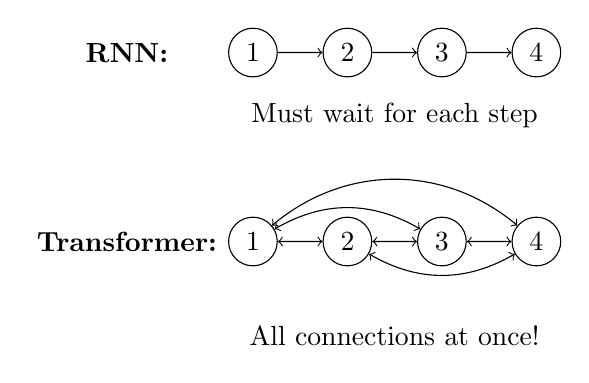
\begin{tikzpicture}[scale=0.8]
    % RNN
    \node at (0, 2) {\textbf{RNN:}};
    \node[circle,draw] (r1) at (2,2) {1};
    \node[circle,draw] (r2) at (3.5,2) {2};
    \node[circle,draw] (r3) at (5,2) {3};
    \node[circle,draw] (r4) at (6.5,2) {4};
    \draw[->] (r1) -- (r2);
    \draw[->] (r2) -- (r3);
    \draw[->] (r3) -- (r4);
    \node at (4.25, 1) {Must wait for each step};
    
    % Transformer
    \node at (0, -1) {\textbf{Transformer:}};
    \node[circle,draw] (t1) at (2,-1) {1};
    \node[circle,draw] (t2) at (3.5,-1) {2};
    \node[circle,draw] (t3) at (5,-1) {3};
    \node[circle,draw] (t4) at (6.5,-1) {4};
    \draw[<->] (t1) -- (t2);
    \draw[<->] (t1) to[bend left=30] (t3);
    \draw[<->] (t1) to[bend left=40] (t4);
    \draw[<->] (t2) -- (t3);
    \draw[<->] (t2) to[bend right=30] (t4);
    \draw[<->] (t3) -- (t4);
    \node at (4.25, -2.5) {All connections at once!};
\end{tikzpicture}
\end{center}

\discovery{
You've identified the key limitation of RNNs: sequential processing prevents parallelization. Transformers process all positions simultaneously!
}

\section{Part 2: Inventing Self-Attention (15 minutes)}

\subsection{The Direct Connection Idea}

\theoryhint{
Instead of information flowing step-by-step through hidden states, what if every word could directly ``attend'' to every other word? This is like giving each word the ability to look at all other words and decide which ones are most relevant to understanding its meaning.
}

\realworld{
Think of attention like a \textbf{spotlight in a theater}:
\begin{itemize}
    \item Each word is an actor on stage
    \item Each actor has a spotlight they control
    \item They can shine their spotlight on other actors (or themselves)
    \item The brightness shows how much they're paying attention
\end{itemize}
}

\exercise{For the sentence ``The cat sat'', draw arrows showing which words should connect:}

\begin{center}
\begin{tikzpicture}[scale=1.5]
    \node at (0,0) {The};
    \node at (2,0) {cat};
    \node at (4,0) {sat};
    % Students draw arrows here
\end{tikzpicture}
\end{center}

\vspace{3em} % Space for drawing

\question{How many connections did you draw? For a sentence with n words, how many connections would we need?}

Connections = \_\_\_\_\_\_\_

\subsection{Computing Relevance}

\theoryhint{
To decide how much one word should ``attend'' to another, we compute a relevance score. These scores are then normalized (using softmax) so they sum to 1.0, creating a probability distribution over the input sequence. This tells us what percentage of attention to give each word.
}

\exercise{For each word pair, assign a relevance score (0-1):}

When processing ``sat'', how relevant is each word?

\begin{center}
\begin{tabular}{|l|c|c|}
\hline
\textbf{Query: ``sat''} & \textbf{Key} & \textbf{Relevance Score} \\
\hline
sat looks at $\rightarrow$ & The & \_\_\_ \\
sat looks at $\rightarrow$ & cat & \_\_\_ \\
sat looks at $\rightarrow$ & sat & \_\_\_ \\
\hline
\textbf{Total} & & Should sum to 1.0 \\
\hline
\end{tabular}
\end{center}

\think{How would you compute these scores mathematically?}

\subsection{The Three Roles: Query, Key, Value}

\theoryhint{
Each word needs to play three distinct roles in attention:
\begin{itemize}
    \item \textbf{Query}: What information am I looking for?
    \item \textbf{Key}: What information do I contain?
    \item \textbf{Value}: What actual content do I provide?
\end{itemize}
This is similar to a database or dictionary lookup system.
}

\realworld{
Imagine a library:
\begin{itemize}
    \item \textbf{Query}: ``I'm looking for books about cats''
    \item \textbf{Key}: Each book's catalog card (title, subject)
    \item \textbf{Value}: The actual book content
\end{itemize}
You compare your query to all keys, then take the values of matching books!
}

\question{Complete the three roles each word plays:}

\begin{enumerate}
    \item \textbf{Q\_\_\_\_\_}: The word asking ``who is relevant to me?''
    \item \textbf{K\_\_\_}: The word answering ``here's what I offer''
    \item \textbf{V\_\_\_\_}: The word providing ``here's my actual information''
\end{enumerate}

\subsection{The Attention Formula}

\theoryhint{
The attention mechanism has four steps:
1. Compute similarity between Query and Keys (dot product)
2. Scale to prevent gradient problems (divide by $\sqrt{d_k}$)
3. Normalize with softmax to get weights summing to 1
4. Weight the Values by these attention weights
}

\exercise{Design the attention mechanism. Fill in the steps:}

\begin{enumerate}
    \item Compute similarity: $Q \times K^T = $ \_\_\_\_\_\_\_
    \item Scale by: $\frac{1}{\sqrt{\_\_\_}}$ (why scale?)
    \item Apply \_\_\_\_\_\_\_ to get weights that sum to 1
    \item Multiply by \_\_\_\_\_ to get final output
\end{enumerate}

\discovery{
Congratulations! You just invented self-attention: 
$$\text{Attention}(Q,K,V) = \text{softmax}\left(\frac{QK^T}{\sqrt{d_k}}\right)V$$
}

\section{Part 3: Why Multiple Heads? (10 minutes)}

\subsection{Different Types of Relationships}

\theoryhint{
A single attention pattern might focus on syntax OR semantics OR position, but rarely all three effectively. By having multiple ``heads'' of attention running in parallel, each can specialize in detecting different types of relationships between words.
}

\realworld{
Like having multiple cameras filming a scene:
\begin{itemize}
    \item Camera 1: Focuses on the main actor (subject)
    \item Camera 2: Captures the action (verb)
    \item Camera 3: Shows the setting (context)
    \item Camera 4: Tracks emotions (sentiment)
\end{itemize}
Each ``head'' captures different relationships!
}

\exercise{Consider the sentence: ``The bank by the river bank''}

First ``bank'' should attend to different words for different reasons:
\begin{itemize}
    \item Syntactic: ``bank'' is a \_\_\_\_\_\_ (noun/verb)
    \item Semantic: ``bank'' means \_\_\_\_\_\_ (financial/shore)  
    \item Position: ``bank'' is the \_\_\_\_\_\_ word
\end{itemize}

\question{Can a single attention pattern capture all these relationships?}

\vspace{2em}

\subsection{Multi-Head Design}

\theoryhint{
Multi-head attention splits the model's representation into multiple subspaces. If we have 8 heads and a model dimension of 512, each head works with 64 dimensions. After each head computes its attention, we concatenate all outputs and mix them with a linear transformation.
}

\think{What if we had multiple attention mechanisms running in parallel, each looking for different patterns?}

\exercise{Design multi-head attention:}

\begin{enumerate}
    \item Number of parallel attentions: \_\_\_\_\_ (typically 8-16)
    \item Each head size: $\frac{d_{model}}{\_\_\_\_\_}$
    \item How to combine outputs: \_\_\_\_\_\_\_\_\_\_\_
\end{enumerate}

Visual example of 4 heads looking at ``bank'':

\begin{center}
\begin{tabular}{|l|l|l|}
\hline
\textbf{Head} & \textbf{Focus} & \textbf{Attends to} \\
\hline
Head 1 & Syntax & ``The'' (determiner) \\
Head 2 & Meaning & ``river'' (context) \\
Head 3 & Position & nearby words \\
Head 4 & Topic & ``water'', ``flow'' \\
\hline
\end{tabular}
\end{center}

\discovery{
Multi-head attention lets the model attend to different types of information simultaneously - syntax, semantics, position, and more!
}

\section{Part 4: The Position Problem (10 minutes)}

\subsection{Order Blindness}

\theoryhint{
Self-attention treats a sentence as a ``bag of words'' - it doesn't inherently know word order. Without position information, ``cat chased mouse'' and ``mouse chased cat'' would look identical to the model. We need to inject position information somehow.
}

\exercise{Self-attention treats these as identical. Why is this a problem?}

\begin{enumerate}
    \item ``The cat chased the mouse''
    \item ``The mouse chased the cat''
\end{enumerate}

Both have the same words, same attention scores between words...

\question{What information is self-attention missing?}

\vspace{2em}

Write two sentences using the same words but different order, where meaning completely changes:

1. \_\_\_\_\_\_\_\_\_\_\_\_\_\_\_\_\_\_\_\_\_\_\_\_\_

2. \_\_\_\_\_\_\_\_\_\_\_\_\_\_\_\_\_\_\_\_\_\_\_\_\_

\subsection{Encoding Position}

\theoryhint{
We need to add position information to each word embedding. The challenge: how to encode positions so that:
\begin{itemize}
    \item Each position is unique
    \item The model can understand relative positions (word 3 is closer to word 4 than to word 10)
    \item It generalizes to sequences longer than training examples
\end{itemize}
}

\think{How can we tell the model about word positions?}

\exercise{Evaluate these approaches:}

\begin{center}
\begin{tabular}{|l|c|c|}
\hline
\textbf{Approach} & \textbf{Pros} & \textbf{Cons} \\
\hline
Add position number [1,2,3...] & Simple & \_\_\_\_\_\_\_ \\
Learn position embeddings & Flexible & \_\_\_\_\_\_\_ \\
Use sin/cos waves & \_\_\_\_\_\_ & Complex \\
\hline
\end{tabular}
\end{center}

\subsection{Sinusoidal Encoding}

\theoryhint{
Sinusoidal (sine/cosine) encodings are clever: they create unique patterns for each position using waves of different frequencies. Lower frequencies change slowly (capturing global position), while higher frequencies change quickly (capturing local distinctions). This allows the model to learn both absolute and relative positions.
}

\realworld{
Like giving each word a unique ``address'':
\begin{itemize}
    \item Position 1: [0.84, 0.54, 0.00, 1.00, ...]
    \item Position 2: [0.91, 0.42, 0.84, 0.54, ...]
    \item Position 3: [0.14, -0.99, 0.91, 0.42, ...]
\end{itemize}
Each position has a unique pattern, like a fingerprint!
}

\question{Why use sine and cosine for positions?}

Properties to achieve:
\begin{itemize}
    \item Each position should be unique
    \item Model should understand relative positions
    \item Should work for any sequence length
\end{itemize}

\exercise{Fill in the position encoding formula:}

$$PE_{(pos, 2i)} = \sin\left(\frac{pos}{10000^{\_\_\_\_\_}}\right)$$
$$PE_{(pos, 2i+1)} = \_\_\_\left(\frac{pos}{10000^{2i/d_{model}}}\right)$$

\discovery{
Sinusoidal position encodings allow the model to learn relative positions and generalize to longer sequences than seen during training!
}

\section{Part 5: Building the Complete Transformer (15 minutes)}

\subsection{The Layer Cake Architecture}

\theoryhint{
A transformer is built from stacking identical layers. Each layer has two main sub-layers:
1. Multi-head self-attention (for looking at other positions)
2. Position-wise feed-forward network (for processing each position independently)
Both use residual connections and layer normalization for stable training.
}

\begin{center}
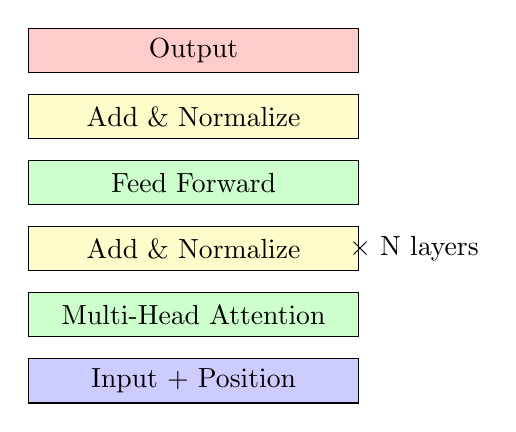
\begin{tikzpicture}[scale=0.7]
    % Input
    \draw[fill=blue!20] (0,0) rectangle (6,0.8);
    \node at (3,0.4) {Input + Position};
    
    % Layer 1
    \draw[fill=green!20] (0,1.2) rectangle (6,2);
    \node at (3,1.6) {Multi-Head Attention};
    
    \draw[fill=yellow!20] (0,2.4) rectangle (6,3.2);
    \node at (3,2.8) {Add \& Normalize};
    
    \draw[fill=green!20] (0,3.6) rectangle (6,4.4);
    \node at (3,4) {Feed Forward};
    
    \draw[fill=yellow!20] (0,4.8) rectangle (6,5.6);
    \node at (3,5.2) {Add \& Normalize};
    
    % Stack indicator
    \node at (7,2.8) {$\times$ N layers};
    
    % Output
    \draw[fill=red!20] (0,6) rectangle (6,6.8);
    \node at (3,6.4) {Output};
\end{tikzpicture}
\end{center}

\exercise{Design one transformer layer. What components do we need?}

\begin{enumerate}
    \item \_\_\_\_\_\_\_\_\_\_\_\_\_\_ (computes attention)
    \item \_\_\_\_\_\_\_\_\_\_\_\_\_\_ (adds shortcut)
    \item \_\_\_\_\_\_\_\_\_\_\_\_\_\_ (normalizes)
    \item \_\_\_\_\_\_\_\_\_\_\_\_\_\_ (processes each position)
    \item \_\_\_\_\_\_\_\_\_\_\_\_\_\_ (another shortcut)
    \item \_\_\_\_\_\_\_\_\_\_\_\_\_\_ (normalizes again)
\end{enumerate}

\subsection{The Feed-Forward Network}

\theoryhint{
After attention aggregates information across positions, we need to process each position individually. The FFN is a simple 2-layer neural network applied to each position separately. It typically expands the dimension (e.g., 512 → 2048) then contracts it back, allowing complex transformations.
}

\question{After attention, why do we need position-wise feed-forward networks?}

Think about:
\begin{itemize}
    \item Attention combines information from different positions
    \item FFN processes \_\_\_\_\_\_\_\_\_\_\_\_\_
\end{itemize}

\subsection{Residual Connections}

\theoryhint{
Residual connections (also called skip connections) add the input directly to the output: $\text{output} = \text{layer}(x) + x$. This creates ``highways'' for gradients to flow backward and information to flow forward, making it possible to train very deep networks.
}

\realworld{
Like having both stairs AND an elevator in a building:
\begin{itemize}
    \item Stairs = Going through the transformation
    \item Elevator = Direct connection (residual)
\end{itemize}
Information can take either path!
}

\exercise{Why add the input to the output (residual/skip connections)?}

Benefits:
\begin{enumerate}
    \item Gradient flow: \_\_\_\_\_\_\_\_\_\_\_
    \item Information preservation: \_\_\_\_\_\_\_\_\_\_\_
    \item Training stability: \_\_\_\_\_\_\_\_\_\_\_
\end{enumerate}

\subsection{Stack and Scale}

\question{If one layer is good, what about many layers?}

\begin{center}
\begin{tabular}{|l|c|c|}
\hline
\textbf{Model} & \textbf{Layers} & \textbf{Parameters} \\
\hline
BERT-Base & 12 & 110M \\
GPT-2 & \_\_\_ & 1.5B \\
GPT-3 & \_\_\_ & 175B \\
\hline
\end{tabular}
\end{center}

\checkpoint{
Like a layer cake, each layer adds more understanding. GPT-3 has 96 layers! Transformers scale exceptionally well - more layers and parameters consistently improve performance.
}

\section{Part 6: Advantages Analysis (10 minutes)}

\subsection{Parallelization}

\theoryhint{
Since all positions can be processed simultaneously, transformers can fully utilize modern parallel hardware (GPUs/TPUs). This is a massive advantage over sequential models.
}

\exercise{Compare processing time:}

100-word sequence:
\begin{itemize}
    \item RNN: 100 sequential steps = \_\_\_\_ time units
    \item Transformer: \_\_\_ parallel step(s) = \_\_\_\_ time unit(s)
\end{itemize}

Speedup factor: \_\_\_\_$\times$

\subsection{Long-Range Dependencies}

\theoryhint{
In RNNs, information must pass through all intermediate steps. In transformers, any word can directly attend to any other word in just one step, making it much easier to capture long-range dependencies.
}

\question{How many steps for word 1 to influence word 100?}

\begin{itemize}
    \item RNN: \_\_\_\_ steps (through all intermediate)
    \item Transformer: \_\_\_\_ step(s) (direct connection)
\end{itemize}

\subsection{Interpretability}

\think{With attention weights, what can we visualize?}

\vspace{3em}

\section{Coding Challenge: Build Your Own Attention}

\theoryhint{
Let's implement the attention mechanism step by step. Remember:
\begin{itemize}
    \item Scores = $Q \times K^T$ (dot product for similarity)
    \item Scale by $\sqrt{d_k}$ to prevent large values
    \item Softmax normalizes scores to sum to 1
    \item Final output weights Values by attention scores
\end{itemize}
}

\begin{lstlisting}[language=Python]
import numpy as np

def softmax(x):
    """Compute softmax values for array x."""
    exp_x = np.exp(x - np.max(x, axis=-1, keepdims=True))
    return exp_x / np.sum(exp_x, axis=-1, keepdims=True)

def self_attention(Q, K, V):
    """
    Compute scaled dot-product attention.
    Q, K, V: matrices of shape (seq_len, d_k)
    Returns: output matrix and attention weights
    """
    d_k = Q.shape[1]
    
    # Step 1: Compute scores (Q x K^T)
    scores = # YOUR CODE: np.dot(Q, K.T)
    
    # Step 2: Scale by sqrt(d_k)
    scores = scores / # YOUR CODE: np.sqrt(d_k)
    
    # Step 3: Apply softmax to get attention weights
    weights = # YOUR CODE: softmax(scores)
    
    # Step 4: Apply weights to values
    output = # YOUR CODE: np.dot(weights, V)
    
    return output, weights

# Test your implementation!
seq_len, d_k = 4, 8
Q = np.random.randn(seq_len, d_k)
K = np.random.randn(seq_len, d_k)
V = np.random.randn(seq_len, d_k)

output, weights = self_attention(Q, K, V)
print("Attention weights shape:", weights.shape)
print("Output shape:", output.shape)
print("Do weights sum to 1?", np.allclose(weights.sum(axis=1), 1))

# Visualize attention weights
print("\nAttention weights (rounded):")
print(np.round(weights, 2))
\end{lstlisting}

\section{Practice Problems}

\subsection{Problem 1: Attention Weights}

\theoryhint{
When filling in attention weights, think about which words are most relevant to each other. Subject words often attend to their verbs, adjectives attend to their nouns, and pronouns attend to what they refer to. Remember: each row must sum to 1.0!
}

Given the sentence ``Dogs love treats'', fill in reasonable attention weights:

\begin{center}
\begin{tabular}{|l|c|c|c|}
\hline
\textbf{From $\downarrow$ To $\rightarrow$} & Dogs & love & treats \\
\hline
Dogs & 0.5 & \_\_\_ & \_\_\_ \\
love & \_\_\_ & 0.2 & \_\_\_ \\
treats & \_\_\_ & \_\_\_ & 0.4 \\
\hline
\end{tabular}
\end{center}

\subsection{Problem 2: Parallelization}

\theoryhint{
RNNs must process sequentially: step 1, then step 2, then step 3, etc. Transformers can process all positions at once. This parallelization is what makes transformers so fast on modern hardware.
}

Calculate the speedup:
\begin{itemize}
    \item Sentence length: 50 words
    \item RNN: Processes 1 word per time step
    \item Transformer: Processes all words at once
\end{itemize}

Time for RNN: \_\_\_\_ steps
Time for Transformer: \_\_\_\_ step(s)
Speedup: \_\_\_\_ times faster

\subsection{Problem 3: Design Challenge}

Design a 2-head attention system for understanding ``Time flies like an arrow'':
\begin{itemize}
    \item Head 1 focuses on: \_\_\_\_\_\_\_\_\_\_\_\_\_
    \item Head 2 focuses on: \_\_\_\_\_\_\_\_\_\_\_\_\_
\end{itemize}

\section{Reflection Questions}

\question{Why is the paper titled ``Attention Is All You Need''?}

\vspace{3em}

\question{What tasks beyond NLP could benefit from transformers?}

\vspace{3em}

\question{What are potential limitations of transformers?}

Think about: computational cost, memory requirements, sequence length limits...

\vspace{3em}

\hrule
\vspace{1em}

\section*{Key Takeaways}

\checkpoint{
Remember these essential points:
\begin{enumerate}
    \item Transformers process all words \textbf{in parallel} (unlike sequential RNNs)
    \item Self-attention creates \textbf{direct connections} between all word pairs
    \item Multiple heads capture \textbf{different types of relationships}
    \item Position encoding tells the model about \textbf{word order}
    \item Residual connections and normalization enable \textbf{deep networks}
    \item This architecture powers \textbf{ChatGPT, BERT, and modern AI}!
\end{enumerate}
}

\section*{Fun Facts}
\begin{itemize}
    \item The transformer paper has been cited over 100,000 times!
    \item GPT-3 would take 355 years to train on a single GPU
    \item Transformers work with images (ViT), music, and even DNA sequences
    \item The original transformer was trained for translation in just 3.5 days
    \item The name comes from ``transforming'' one sequence to another
\end{itemize}

\section*{Next Steps}
\begin{enumerate}
    \item Try the Jupyter notebook to build your own transformer
    \item Experiment with attention visualizations
    \item Explore pre-trained models next week
    \item Challenge: Read ``Attention Is All You Need'' paper
\end{enumerate}

\realworld{
You now understand the architecture that revolutionized AI. These concepts you discovered today power ChatGPT, BERT, and virtually all modern NLP systems. You're ready to dive deeper into the world of transformers!
}

\vspace{2em}
\noindent\textbf{Next Week:} We'll explore pre-trained language models (BERT, GPT) and the revolution they started!

\end{document}